\documentclass{article}
\usepackage[utf8]{inputenc}
\usepackage{mathpazo} % Palatino font
\usepackage{natbib}
\usepackage{graphicx}
\usepackage{enumitem}
\usepackage{amsmath}
\usepackage{amssymb}
\usepackage{ragged2e}
\usepackage{subfig}
\usepackage{algorithm}
\usepackage{algorithmic}
\usepackage{diagbox}
\usepackage[textwidth=12.7cm]{geometry}


\usepackage{xcolor}
\newcommand\todo[1]{\textcolor{red}{#1}}

\bibliographystyle{abbrv} %format des citations

\begin{document}
\begin{titlepage}
	\newcommand{\HRule}{\rule{\linewidth}{0.5mm}}
					
	\center
					
	\textsc{\LARGE Université de Bordeaux}\\[1.5cm]
					
	\textsc{\Large Master 1 Informatique}\\[0.5cm]
					
	\textsc{\large Projet de programmation}\\[0.5cm]
					
	\HRule\\[0.4cm]
					
	{\huge\bfseries Génération de playlistes musicales pour un groupe d'utilisateurs}\\[0.4cm]
	{\Large\bfseries Cahier d'analyse des besoins}
	\HRule\\[1.5cm]
					
	\begin{minipage}{0.4\textwidth}
			
		\begin{flushleft}
			\large
			\textit{Client}\\
			\textsc{Hanna}  Pierre 
		\end{flushleft}
				
		\begin{flushleft}
			\large
			\textit{Chargé de TD}\\
			\textsc{Boussicault}  Adrien 
		\end{flushleft}
				
		\begin{flushleft}
			\large
			\textit{Auteurs}\\
			\textsc{Amadou Bah}  Elhajd 
			\\
			\textsc{Deguillaume} Nicolas
			\\
			\textsc{Jolliet} Louis
			\\
			\textsc{Loison} Jules 
			\\
			\textsc{Vigneau} Paul 
		\end{flushleft}
				
	\end{minipage}
	\vfill\vfill\vfill
					
	{\large 4 Février 2020}
	\vfill\vfill
	
\includegraphics[width=0.5\textwidth]{ressources/Logo.jpg}\\[1cm]
		\vfill
		\end{titlepage}
		\justify
		\renewcommand{\contentsname}{Table des matières}
		\tableofcontents
		\newpage
								
		\section{Introduction au projet}
		\paragraph{}
		Notre client souhaite une application qui permet de générer des playlists de titres musicaux qui plairaient à un groupe composé d'un certain nombre d'utilisateurs en utilisant l'API de Spotify ou Deezer. L'intérêt principal de ce projet est de créer un produit qui puisse être utilisé par des chercheurs du LaBRI, leur permettant de tester différents algorithmes. En effet l'application doit proposer un ou plusieurs algorithmes ayant pour but de générer des playlists composées de musiques plaisant le plus possible à tous les utilisateurs. Pour ce faire, l'application doit récupérer les informations d'écoute de ces utilisateurs (musiques appréciées, playlists personnelles, genres les plus écoutés, etc). 
								    
		Ensuite, l'application doit permettre à l'utilisateur d'écouter cette playlist nouvellement générée, en embarquant un lecteur de musique comprenant des options basiques telles que changer de musique, faire pause, reprendre, mettre un "j'aime", etc. L'application doit pouvoir récupérer les logs d'écoute (chaque interaction avec le lecteur) afin de pouvoir analyser et évaluer les différents algorithmes. Une fois l'application produite, les chercheurs du LaBRI pourront ensuite ajouter et analyser de nouveaux algorithmes plus complexes, mais nous devons néanmoins en implémenter. 
								    
		Enfin, des points importants soulignés par le client, destinés à nous guider au moment de prendre certains choix d'implémentation, sont que le produit doit être assez intuitif, rapide et simple d'utilisation. 
								
		Nous avons choisi d'utiliser l'API de Spotify afin de réaliser l'application car nous sommes plus familiers avec ce service.     
								
		\subsection{Descriptions des termes}
		\begin{itemize}
			\item Track : titre de musique
			\item Playlist : liste de titres de musique. Dans ce document on ajoutera souvent un adjectif à la suite du mot \textit{playlist} parmi les suivants : 
			      \begin{itemize}
			      	\item Personnelle : playlist enregistrée sur le compte d'un utilisateur en particulier 
			      	\item Locale : playlist créée sur notre application et qui n'existe que dans cette-ci. Elle n'existe sur aucun compte utilisateur
			      	\item Publique : visibilité d'une playlist personnelle. Elle est visible (écoutable) par n'importe quel utilisateur
			      	\item Privée : visiblité d'une playlist personnelle. Elle n'est visible (écoutable) que par l'utilisateur qui a enregistré cette playlist
			      \end{itemize} \newpage
			\item Utilisateur : personne physique détentrice d'un compte Spotify ou Deezer. Dans ce document on ajoutera souvent un adjectif à la suite du mot \textit{utilisateur} parmi les suivants:
			      \begin{itemize}
			      	\item Authentifié ou principal (main user) : utilisateur qui a autorisé notre application à utiliser son compte Spotify ou Deezer afin d'effectuer des requêtes
			      	\item Utilisateur courant (current user) : utilisateur qui a l'appareil en main et qui s'est désigné comme celui qui interagit avec l'application
			      	\item Utilisateur secondaire (other user) : utilisateur qui a renseigné son nom d'utilisateur afin de s'ajouter au groupe
			      \end{itemize}
			\item Session d'écoute : moment durant lequel les titres de la playlist locale sont en écoute
		\end{itemize}
				
		\subsection{Acteurs}
		\begin{itemize}
			\item Utilisateurs: principal, secondaires ou courants, ils utilisent et interagissent avec l'application
			\item Serveur: il envoie la requête d'authenfication à l'API afin de récupérer un jeton d'accès (\textit{access\_token}) que  notre application (client) récupère afin de l'utiliser dans ses requêtes. Il sert aussi à avoir un rafraichissement automatique du jeton toutes les heures. Avoir un service en backend est nécessaire car, afin de récupérer un \textit{access\_token}, il faut envoyer la clé secrète de notre application dans la requête d'authentification. Ainsi, pour des raisons de sécurité on ne peut pas permettre au client de connaître la clé secrète et donc d'envoyer la requête d'authentification
			\item API Spotify/Deezer: API que l'on sollicite à chaque requête afin d'accéder aux informations des utilisateurs ainsi qu'à des fonctionnalités comme la création de playlists personnelles ou la modification de celles-ci
		\end{itemize}

		\section{Description et analyse de l'existant}
		\paragraph{}
		Nous démarrons notre application de zéro, cependant il existe certains exemples nous permettant d'avoir des idées de fonctionnalités ou de design. Pour le moment, les seuls exemples dont nous pouvons nous inspirer qui correspondent le plus à ce que nous devons réaliser sont Friends Mix par Apple et Family Mix par Spotify. En effet, Apple Music propose un mix, renouvelé chaque semaine incluant les 25 chansons les plus écoutées par nos amis. De la même façon, Spotify, dans leur offre Premium Family (pouvoir avoir jusqu'à 6 utilisateurs sur un même compte), offre une playlist incluant les goûts de chacun. Ces applications possèdent un certain nombre des fonctionnalités énoncées en \ref{besoins}, il est bien sûr impossible de customiser l'algorithme de génération des playlists, ce qui est le but premier de notre client. Nous pouvons cependant nous inspirer de certaines fonctionnalités disponibles et pouvons améliorer l'expérience utilisateur, tel que la provenance des musiques (de quel(s) utilisateur(s) provient la musique) comme on peut le voir sur la Figure \ref{fig:example}.
								
								
		De plus nous allons nous servir de différents dépots GitHub utilisant les API Spotify \cite{spotify-web-api} ou Deezer.
								
		\begin{figure}[hb!]
			\centering
			\subfloat[Friends Mix - Apple Music]{{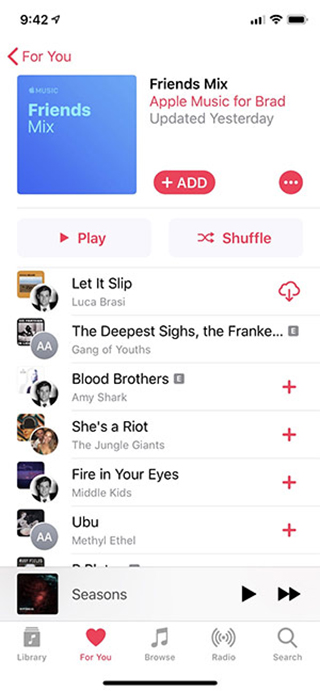
\includegraphics[width=5cm]{ressources/friends-mix-apple-music.jpg} }}%
			\qquad
			\subfloat[Family Mix - Spotify]{{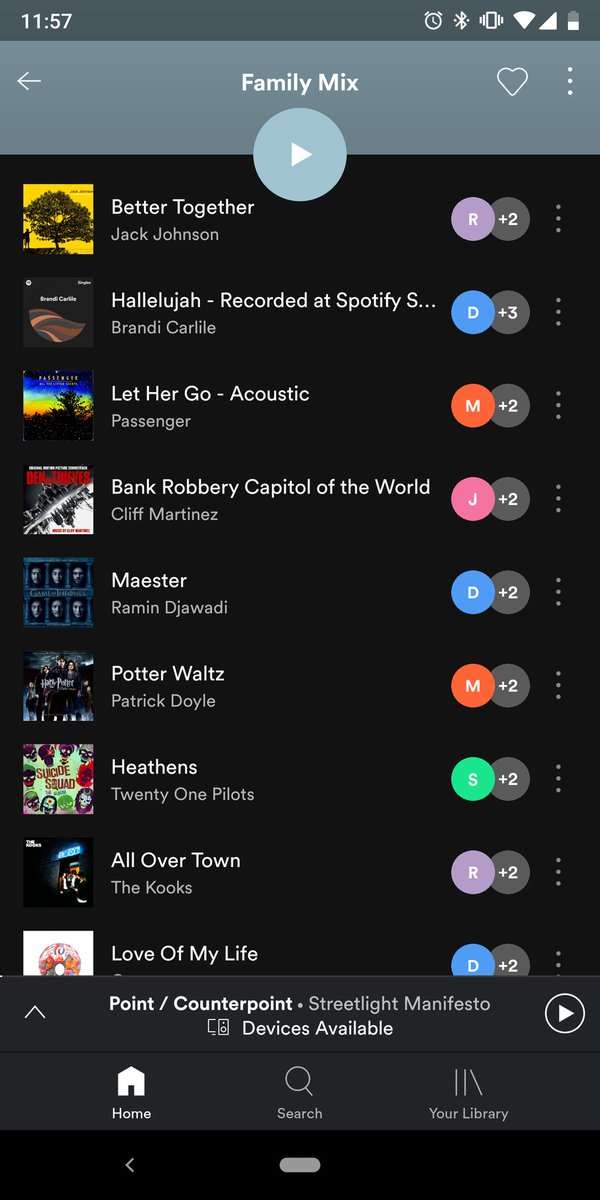
\includegraphics[width=5cm]{ressources/Spotify_Family_Mix.jpg} }}%
			\caption{Exemple d'applications similaires}%
			\label{fig:example}%
		\end{figure}
		\newpage		
		\section{Description des besoins} \label{besoins}
		Afin de décrire la priorité de chaque besoin, nous écrirons au début de la description d'un besoin un de ces mots :
		\begin{itemize}
			\item \textbf{Essentiel} : le logiciel ne sera pas acceptable sans que ce besoin ne soit réalisé
			\item \textbf{Conditionnel} : besoin qui étend et améliore le logiciel, sans que ce besoin soit nécessaire pour rendre le logiciel acceptable
			\item \textbf{Optionnel} : besoin dont la valeur n’est pas encore assurée. Donne au fournisseur l’occasion de proposer quelque chose qui va au-delà des besoins attendus
		\end{itemize}
		\subsection{Besoins fonctionnels}
		Nous détaillerons les besoins suivants, exprimés par le client :
		\subsubsection{Choisir une plateforme de streaming musical sur laquelle s'interfacer}
		\textbf{[ Essentiel ]}
		\begin{itemize}
			\item Pouvoir choisir d'utiliser l'API de Spotify au démarrage de l'application
		\end{itemize}
		\textbf{[ Optionnel ]}
		\begin{itemize}
			\item Pouvoir choisir d'utiliser l'API de Deezer au démarrage de l'application
		\end{itemize}
		\subsubsection{Authentifier l'utilisateur principal} \label{authentification}
		\textbf{[ Essentiel ]}
		\begin{itemize}
			\item Après avoir choisi quelle API utiliser, un utilisateur doit pouvoir s'authentifier
		\end{itemize}
		\textbf{Test du besoins} 
		\begin{itemize}
			\item On s'authentifie au début du test. On vérifie ensuite que l'authentification s'est bien passée ainsi que le bon fonctionnement des requêtes. Pour cela nous envoyons la requête suivante: \textit{GET https://api.spotify.com/v1/me} pour récupérer le profil de l'utilisateur authentifié. On regarde ensuite le code de retour de la requête. Si le code de retour est 200, cela signifie que la requête a réussi et que donc l'authentification aussi (car cette requête récupère les informations de l'utilisateur authentifié): le test réussit. Si le code de retour est 401, cela signifie que l'authentification a échouée : le test échoue
		\end{itemize}
		\newpage
		\subsubsection{Créer un groupe d'utilisateurs}
		\textbf{[ Essentiel ]}
		\begin{itemize}
			\item Réussir l'authentification crée un groupe d'utilisateurs contenant intialement seulement l'utilisateur principal
		\end{itemize}
		\subsubsection{Ajouter des membres secondaires au groupe}  \label{connexion}
		\textbf{[ Essentiel ]}
		\begin{itemize}
			\item Cliquer sur un bouton et renseigner un identifiant utilisateur dans une boîte de texte permet d'ajouter un utilisateur au groupe
		\end{itemize}
		\textbf{Test du besoin} 
		\begin{itemize}
			\item On renseigne des identifiants utilisateur (id) au début du test. Pour chaque id renseigné, on envoie la requête \textit{GET https://api.spotify.com/v1/users/\{id\}} pour récupérer le profil de chaque utilisateur. On regarde ensuite le code de retour de la requête. Si le code de retour est 200, cela signifie que la requête a réussi: le test réussit. Si le code de retour de la requête est 404, cela signifie que l'utilisateur n'existe pas, le test échoue
		\end{itemize}
		\subsubsection{Supprimer des membres du groupe}
		\textbf{[ Conditionnel ]}
		\begin{itemize}
			\item Supprimer l'utilisateur principal le fera se déconnecter et supprimera la session d'écoute et le groupe
		\end{itemize}
		\textbf{[ Optionnel ]}
		\begin{itemize}
			\item Un utilisateur secondaire doit pouvoir être supprimé du groupe
		\end{itemize}
						            
		\subsubsection{Ignorer un utilisateur dans la génération de playlist}
		\textbf{[ Optionnel ]}
		\begin{itemize}
			\item Un utilisateur doit pouvoir être ignoré dans l'algorithme (fonction "mute") : ses données ne seront pas utilisées pour le calcul de la playlist locale (cf. \ref{interface_utilisateur} (c))
		\end{itemize}
		\newpage		            
		\subsubsection{Accès aux informations de chaque utilisateur} 
		Une fois un utilisateur ajouté au groupe (cf. \ref{authentification} ou \ref{connexion}), il faut accéder à ses chansons préférées via l'API choisie. 
		\newline \\
		\textbf{[ Essentiel ]}
		\begin{itemize}
			\item Récupérer et charger en mémoire les playlists publiques des utilisateurs au format JSON via l'API
		\end{itemize}
		\textbf{Test du besoin}
		\begin{itemize}
			\item On s'authentifie et on renseigne des identifiants utilisateur (id) au début du test. Pour chaque id renseigné, on envoie la requête \newline\textit{GET https://api.spotify.com/v1/users/\{id\}/playlists} pour récupérer les playlists de chaque utilisateur. Si le code de retour de la requête est 404, cela signifie que l'utilisateur n'existe pas: le test échoue. Si le code de retour de la requête est 200, on continue le test. On envoie ensuite la requête \textit{ GET https://api.spotify.com/v1/me/playlists} pour récupérer les playlists de l'utilisateur authentifié. Si le code de retour de la requête est 200 le test réussit, sinon le test échoue. \newline
			      Tous les tests qui nécessitent les playlists les récupèrent au début du test de la même manière que dans ce test
		\end{itemize}
		\textbf{[ Conditionnel ]} \label{connexion de tous les utilisateurs}
		\begin{itemize}
			\item Récupérer et charger en mémoire d'autres informations (sous format JSON) comme les chansons aimées ou artistes préférés. Cependant ces informations étant privées, cela nécessite d'implémenter une connexion de tout les utilisateurs.\\
			Il n'est pas possible de connecter réellement plusieurs comptes sur la même application. En effet, lors de l'authentification au service de Spotify par un utilisateur, le serveur (de l'API) et le client (l'application, le navigateur, etc) gardent des informations garantissant à l'utilisateur une connexion stable. Il peut donc exécuter des requêtes afin de récupérer des informations privées sur son compte.\\
			Si un autre utilisateur se connecte via la même application (imaginons que cela soit implémenté), cela va avoir pour conséquence de déconnecter l'utilisateur précédent - ou du moins d'écraser les données stockées sur le serveur et le client. L'envoi d'une requête visant à obtenir des informations privées va donc retourner des données relatives au deuxième compte.\\
			Une solution possible serait de permettre l'authentification de plusieurs comptes, mais à chaque connexion, de récupérer toutes les informations nécessaires au bon fonctionnement de l'application et de les stocker. L'application se servirait donc du dernier utilisateur connecté pour exécuter des requêtes vers l'API mais disposerait des informations de tous les comptes précédemment enregistrés.\\
			Cette solution n'est qu'une supposition de ce qu'il est possible de faire. Il n'y a eu aucun prototype visant à tester cette fonctionnalité.
		\end{itemize}
		\subsubsection{Proposition de playlist(s)}
		\textbf{[ Essentiel ]}
		\begin{itemize}
			\item L'utilisateur doit pouvoir lancer un mix (ce qui aura pour effet de lancer l'algorithme puis lancer automatiquement l'écoute de la première chanson)
			\item L'application devra pouvoir créer une playlist vide
			\item L'application devra pouvoir ajouter les titres retournés par l'algorithme à cette playlist locale
		\end{itemize}
		\textbf{Test des besoins}
		\begin{itemize}
			\item On s'authentifie, on renseigne des identifiants utilisateur (id) et on récupère les playlists des utilisateurs au début du test. On crée une playlist, représentée par une structure de données sur laquelle on effectue un test pour savoir si elle est de taille 0 si c'est le cas le test continue, dans le cas contraire il échoue. On fait tourner l'algorithme de génération de playlist. On ajoute ces titres à la structure de données représentant la playlist. On teste si la taille de la playlist est de taille \textit{n} (\textit{n} étant le nombre de musiques générées). Si c'est le cas, le test réussit, sinon il échoue
		\end{itemize}
		\textbf{[ Optionnel ]}
		\begin{itemize}
			\item Pouvoir ajouter les playlists au compte Spotify de l'utilisateur principal
			\item Pouvoir renseigner sur l'application des données qui seront incluses à la requête de création de playlist personnelle : 
			      \begin{itemize}
			      	\item Nom : renseigne le nom de la playlist (chaîne de caractères)
			      	\item Visibilité : définit si la playlist est privée ou publique (booléen, \textit{true} pour publique et \textit{false} pour privée)
			      	\item Collaboration : définit si la playlist est collaborative ou pas (booléen). Pour qu'une playlist soit collaborative, il faut qu'elle soit privée.
			      	\item Description : renseigne la description de la playlist (chaîne de caractères)
			      \end{itemize}
		\end{itemize}
		\textbf{Test du besoin}
		\begin{itemize}
			\item On s'authentifie, on renseigne des identifiants utilisateur (id) et on récupère les playlists des utilisateurs au début du test. On envoie la requête \textit{POST https://api.spotify.com/v1/users/\{id\}/playlists} pour créer une playlist sur le compte de l'utilisateur authentifié (id doit donc être son identifiant utilisateur). On envoie ensuite les requêtes \textit{POST https://api.spotify.com/v1/playlists/\{playlist\_id\}\newline/tracks} en renseignant l'identifiant des musiques à ajouter. Si le code de retour des requêtes est 200 le test réussit, sinon le test échoue.
		\end{itemize}
		\subsubsection{Proposer différents algorithmes de génération de playlists}\label{algos}
		\textbf{[ Essentiel ]}
		\begin{itemize}
			\item  L'application implémentera un algorithme naïf qui proposera des musiques prises au hasard dans les playlists publiques des utilisateurs.\newline \\
			      Le premier algorithme que nous allons implémenter est un algorithme de test, dit naïf qui sera utilisé pour tester l'achitecture que nous avons choisie (cf. \ref{archi_log}). Il consistera à récupérer un nombre égal de musiques provenant des playlists publiques de chaque utilisateur, sans critère particulier. Ce nombre sera défini comme la taille maximale d'une playlist locale (cf. \ref{performance}) divisée par le nombre d'utilisateurs.
			      		
		      \item  L'application proposera au moins un algorithme \cite{ICDM2017} permettant de tester les fonctionnalités proposées par le produit final.\newline \\
		            Le premier algorithme à implémenter consiste à analyser les chansons des playlists publiques grâce au service \textit{Audio Features and Analysis} de l'API Spotify \cite{spotify-web-api}. Celle-ci permet d'obtenir des données sur une chanson comme son degré d'acoustique, son tempo, son énergie, etc. Nous allons par la suite analyser ces données \cite{Data_analysis} en effectuant les opérations suivantes : 
		            \begin{itemize}
		                \item Profil type de chaque utilisateur en effectuant la moyenne des données de chaque titre
		                \item La différence des moyennes entre utilisateurs
		                \item Observer la diversification des utilisateurs (est-ce qu'un utilisateur écoute des musiques diversifiées selon les données) 
		            \end{itemize}
		            Cela permet de mettre en valeur les données les plus importantes pour chaque utilisateur. Par la suite, on compare ce profil type de chaque utilisateur sur toutes les musiques de toutes les playlists et on attribut un score en fonction de l'écart entre les deux valeurs.
		            On obtient donc un score par musique et par utilisateur. \\
		            Par la suite, on attribut un score final à chaque musique en utilisant la \textit{Least Misery Strategy} \cite{Masthof2011} qui est une stratégie d'évaluation qui évalue un item avec le plus bas score qu'un utilisateur lui a attribué. De cette façon, il n'y aura pas de chanson détestée par un utilisateur dans la playlist générée.
			      
			\item L'application proposera de changer d'algorithme dans les options (car le client pourra ajouter des algorithmes)
		\end{itemize} 
		\newpage
		\textbf{[ Conditionnel ]}
		\begin{itemize}
			\item  L'application proposera d'autres algorithmes \cite{ICDM2017} plus complexes permettant une réelle analyse des données. \newline \\
			      Le second algorithme que nous implémenterons se base sur un autre article scientifique \cite{Masthof2011} qui met en avant la notation des éléments pour déterminer comment les proposer à un groupe d'utilisateurs. Cet algorithme nécessite la réalisation du besoin fonctionnel conditionnel d'authentification de tous les utilisateurs (cf. \ref{connexion de tous les utilisateurs}) pour être implémenté. \newline
			      Spotify ne propose pas de système de notation des chansons pour chaque utilisateur. Il nous faut donc attribuer nous même un score à chaque titre en fonction des données récupérées des utilisateurs. On récupère les 50 (limite de la requête) titres les plus écoutés de chaque utilisateur. On cherche ensuite à affecter un score à chacun des titres en fonction de plusieurs critères : 
			      \begin{itemize}
			      	\item Classement des titres en terme d'écoute
			      	\item Si un titre est dans la liste des titres préférés d'autres utilisateurs
			      	\item Si un titre dans la liste d'un utilisateur a le même artiste qu'un titre de la liste d'un autre utilisateur (et que les titres ne sont pas les mêmes)
			      \end{itemize}
			      Une fois ce classement terminé, on a \textit{50 * nombre d'utilisateurs dans le groupe} titres à partir desquels créer la playlist locale. On sélectionne les \textit{x} premiers titres qui ont le score le plus élevé. Avec \textit{x} étant la taille maximale de la playlist locale (cf. \ref{performance}).
		\end{itemize}
		\newpage
		\subsubsection{Lecture de la playlist locale, avec possibilité de skipper des titres} \label{lecture}
		\textbf{[ Essentiel ]} 
		\begin{itemize}
			\item L'utilisateur pourra écouter des chansons et pourra effectuer les interactions suivantes :
			      \begin{itemize}
			      	\item Resume/pause
			      	\item NextTrack/previousTrack
			      	\item Like
			      \end{itemize}
		\end{itemize}
		\textbf{Tests du besoin}
		\begin{itemize}
			\item On s’authentifie. On initialise le lecteur (SDK). On ajoute un \textit{EventListener} sur l'évènement \textit{ready} et sur l'évènement \textit{not\_ready}. Si le premier évènement est déclenché on peut continuer le test, si le second l'est le test échoue. On ajoute un \textit{EventListener click} sur le bouton \textit{like} et sur l'évènement \textit{player\_state\_changed} qui est appelé dès que l'état du lecteur change, l'API nous retourne alors un objet contenant diverses informations sur la session. On lance 3 musiques. On met en pause, on vérifie que la variable \textit{paused} est \textit{true}. On relance la musique, on vérifie que la variable \textit{paused} est \textit{false}. On vérifie que la musique jouée est la 1ère des 3. On vérifie que la musique suivante est la 2ème. On accède à la musique suivante. On vérifie que la musique actuelle est la 2ème, que la musique précédente est la 1ère et que la suivante est la 3. On accède à la musique précédente. On vérifie que la musique actuelle est la 1 et que la musique suivante est la 2. On  \textit{like} le titre. On vérifie que l'on est bien passé dans l'évènement du \textit{like}. Si toutes les vérifications sont passées, c'est que le test réussit. Si une vérification ne passe pas, le test échoue
		\end{itemize}
		\textbf{[ Conditionnel ]}
		\begin{itemize}
			\item L'utilisateur courant est visible en haut de l'application (cf. \ref{interface_utilisateur} (b)) 
			\item L'utilisateur physique pourra choisir qui est l'utilisateur courant (pour pouvoir associer les interactions précédemment énoncées à un utilisateur). Pour cela il devra cliquer sur l'icône utilisateur, puis sélectionner l'utilisateur courant. Cela aura pour utilité d'identifier l'utilisateur qui interagit avec l'application
		\end{itemize}
		\textbf{[ Optionnel ]}
		\begin{itemize}
			\item L'utilisateur pourra se déplacer dans une chanson via une pop-up qui s'affichera en cliquant sur la chanson en cours. 
			\item Cette pop-up fera apparaître l'ensemble des options précédemment présentées (cf. \ref{lecture})
		\end{itemize}
		\newpage
		\subsubsection{Récupération des logs d'écoute pour évaluation des algorithmes} \label{logs}
		\textbf{[ Essentiel ]}
		\begin{itemize}
			\item Ce besoin peut se découper en plusieurs sous-besoins :
			      \begin{itemize}
			      	\item Récupérer et charger en mémoire les méta-données (cf. \ref{WebPlaybackState_Object}) correspondant aux interactions de la session d'écoute (cf. \ref{lecture}) grâce au WEB Player SDK et au bouton like
			      	\item Créer un fichier JSON sur l'appareil de l'utilisateur
			      	\item Y renseigner les méta-données précédemment stockées en mémoire
			      \end{itemize}
		\end{itemize}
		\textbf{Tests du besoin}
		\begin{itemize}
			\item On s'authentifie. On initialise le lecteur (SDK). On ajoute les mêmes  \textit{EventListener} que dans le test précédent. On simule les mêmes interactions que dans le test précédent. A chaque interaction on vérifie qu'elle s'est bien ajoutée à l'object JSON. On vérifie que l'object JSON final a le contenu qui correspond aux interactions. On crée un fichier JSON, on vérifie si le fichier JSON a bien été créé. On écrit dans le fichier le contenu de l'objet JSON, on vérifie que le contenu du fichier et de l'objet sont les mêmes. Si toutes les vérifications sont passées, c’est que le test réussit. Si une vérification ne passe pas, le test échoue
		\end{itemize}
		\textbf{[ Conditionnel ]}
		\begin{itemize}
			\item Ajout de l'utilisateur qui effectue l'interaction recensée par le log. (Va de paire avec les besoins conditionnels du \ref{lecture})
		\end{itemize}
		\textbf{[ Optionnel ]}
		\begin{itemize}
			\item Envoi du fichier par email pour que le client obtienne les logs automatiquement, sans contact avec l'utilisateur ou stockage des fichiers du log sur le serveur
		\end{itemize}
		\subsubsection{Accord d'utilisation de données}
		\textbf{[ Essentiel ]}
		\begin{itemize}
			\item L'application s'ouvrira affichant les conditions d'utilisation. Il sera alors demandé aux utilisateurs leur accord pour collecter les logs d'utilisation de l'application
		\end{itemize}
		\newpage
		\subsection{Besoins non fonctionnels}
		\subsubsection{Performance} \label{performance}
		\textbf{[ Essentiel ]}
		\begin{itemize}
			\item La génération d'une playlist, suivie du lancement de la première musique ne doit pas dépasser 3 secondes. En effet d'après une étude menée en 2018 \cite{MobileSpeedGoogle2018}, l'utilisateur à 53\% de chance de quitter l'application passé ce délai.
			      			
			\item Les complexités des algorithmes proposés en \ref{algos} sont les suivantes : \newline
			      Posons les variables suivantes pour calculer la complexité : 
			      \begin{itemize}
			      	\item[] \textbf{U} : le nombre d'utilisateurs connectés à l'application
			      	\item[] \textbf{N} : le nombre de chansons récupérées par utilisateur
			      \end{itemize}
			      \begin{itemize}
			      	\item Algorithme naïf : il s'agit d'un simple parcours de liste, avec une complexité \textbf{$O(N*U)$}
			      	\item Premier algorithme : Pour l'analyse des données, on obtient une complexité de \textbf{$O(U*N)$}. Pour la comparaison avec chaque titre, on obtient \textbf{$O(U^2*N)$}. Cet algorithme a donc une complexité de \textbf{$O(U^2*N)$}
			      	\item Second algorithme : les requêtes effectuées pour cet algorithme renvoient une liste de titres, d'une taille maximale de \textit{50 titres}. Le parcours d'une liste nous donne donc une complexité de \textbf{$O(1)$}. On parcourt également l'ensemble des listes pour comparer les titres : on obtient donc une complexité de \textbf{$O(U^2)$}
			      	      		
			      \end{itemize}
			\item Sur Spotify, les playlists peuvent contenir jusqu'à 10 000 titres néanmoins nous ne les générerons qu'avec 25 titres pour commencer tout comme le fait Apple Music avec son Friends Mix. Le chiffre pourra éventuellement grandir dans le futur en fonction des performances de notre application et des algorithmes utilisés. (cf. \ref{performance})
		\end{itemize}
		\subsubsection{Portabilité}
		\textbf{[ Essentiel ]}
		\begin{itemize}
			\item L'application devra fonctionner sur la majorité des versions d'Android à savoir celles supérieures à Android 6 Marshmallow soit ~75\% des versions couramment utilisées \cite{AndroidVersion2019}
		\end{itemize}
		\textbf{[ Optionnel ]}
		\begin{itemize}
			\item L'application devra fonctionner sur la majorité des versions d'iOS à savoir celles supérieures à iOS 12 soit ~90\% des versions couramment utilisées d'après Apple  \cite{iOSVersion2019}
		\end{itemize}
		\subsubsection{Planning}
						
		Le planning général nous est imposé durant ce projet, notamment la série d'échéances suivante : 
		\begin{itemize}
			\item	   1ere release : Vendredi 14 Février
			\item	  Audits : Mercredi 19 Février
			\item	   Mémoire et release Finale du code : Jeudi 02 Avril
			\item	  Soutenances : Mercredi 08 Avril
		\end{itemize}
		Le développement durera donc 10 semaines et aura lieu entre la semaine 6 (3 Février) et 14 (2 Avril).
						            
						
								   
		\subsection{Scénarios, prototypes, schémas et diagrammes UML}
		\subsubsection{Scénarios}
		Connexion d'un utilisateur principal :
		\begin{itemize}
			\item L'utilisateur lance l'application
			\item Il arrive sur une page lui proposant de se connecter à Spotify
			\item Il rentre son identifiant et son mot de passe puis confirme
			\item Si l'utilisateur est reconnu par Spotify, l'application le redirige vers la page principale
			\item Sinon, la page lui informe qu'il a fait une erreur dans la saisie
		\end{itemize}
		Ajout d'un utilisateur secondaire :
		\begin{itemize}
			\item[] \textbf{Contexte} : l'utilisateur principal est connecté et il est sur la page principale de l'application.
			\item L'utilisateur clique sur le bouton "plus" situé dans la barre de navigation en haut de l'écran
			\item Une pop-up apparaît avec un champ de texte
			\item L'utilisateur entre l'identifiant du compte Spotify à ajouter et valide
			\item Si l'identifiant est correct, le nouvel utilisateur est ajouté au groupe et la pop-up disparaît
			\item Sinon, l'application indique que l'identifiant est erroné
		\end{itemize}
		\newpage
		Écoute d'une playlist : (algorithme par défaut)
		\begin{itemize}
			\item[] \textbf{Contexte} : Un utilisateur principal est connecté, il a ajouté ou non des utilisateurs secondaires et l'application est sur la page principale.
			\item L'utilisateur clique sur le bouton \textit{MIX} (cf. \ref{interface_utilisateur} (b))
			\item Un traitement se fait alors et affiche tous les titres présents dans la playlist ainsi générée
			\item Automatiquement, le premier titre de la playlist se lance
		\end{itemize}
		Changement de l'algorithme de génération de playlist :
		\begin{itemize}
			\item[] \textbf{Contexte} : Un utilisateur principal est connecté et il se trouve sur la plage principale.
			\item L'utilisateur clique sur l'icône en forme d'engrenage (cf. \ref{interface_utilisateur} (b))
			\item Il se retrouve sur la page des paramètres
			\item Il cherche la partie affichant l'algorithme choisi et appuie dessus
			\item Une liste des algorithmes proposés s'affiche alors
			\item Il sélectionne celui de son choix
			\item La liste se ferme et l'algorithme est automatiquement changé
		\end{itemize}
		Ne pas prendre en compte un membre lors de la génération d'une playlist (fonctionnalité "mute") :
		\begin{itemize}
			\item[] \textbf{Contexte} : Un utilisateur principal est connecté, il a ajouté au moins un membre secondaire et l'application est sur la page principale.
			\item L'utilisateur clique sur l'icône en forme d'engrenage (cf. \ref{interface_utilisateur} (b))
			\item Il se retrouve sur la page des paramètres
			\item Une partie dédiée à l'affichage des membres se trouve dans la page
			\item Il clique sur "Gestion des utilisateurs" et il est redirigé vers une nouvelle page
			\item À côté de chaque membre se trouve un bouton "switch"
			\item Il peut donc désactiver la ou les personnes de son choix
			\item À chaque interaction, son action est sauvegardée
		\end{itemize}
								
		\subsubsection{Prototypes}\label{prototype}
								
		Dans un premier temps, nous avons étudié la documentation de l'API de Spotify. Elle fonctionne de la manière suivante : l'application envoie une requête aux services de l'API Spotify et cette dernière répond au format JSON. Avant tout accès à l'API, il faut au préalable s'authentifier auprès de celle-ci.
								
		\paragraph{Authentification}\mbox{}
								
		Nous avons donc cherché dans un premier temps comment se connecter à Spotify. Il existe une technique simple et très pratique pour se familiariser avec les fonctionnalités que propose l'API, il suffit juste de récupérer dans son compte (sur le site développeur de Spotify) un jeton (\textit{token}). Ce jeton sert de clé d'authentification et il suffit de le renseigner à chaque appel à l'API. Malheureusement, cette méthode présente plusieurs points négatifs pour le produit final, le premier est qu'il faut systématiquement récupérer sur le site de Spotify un jeton et le rentrer dans l'appli-\newline cation (ce qui éloigne le côté facile d'utilisation de l'application). Le deuxième point est que ce jeton est valable uniquement une heure.
								
		Il a donc fallu trouver une méthode plus pratique d'un point de vue utilisateur car ce dernier n'a pas de compte développeur Spotify ni l'envie de devoir chercher puis rentrer un jeton dans l'application pour s'en servir. Nous avons donc découvert que Spotify permet de générer un jeton en se connectant à son compte au travers d'un formulaire (identique à la connexion au service classique). Cette connexion retourne à l'application le jeton nécessaire aux appels API. Ce jeton est valable une heure comme pour la méthode précédente, mais il est accompagné d'un jeton de rafraîchissement (\textit{refresh\_token}) permettant de refaire une demande de jeton sans avoir à forcer l'utilisateur à se connecter à nouveau.
								
		\paragraph{Récupération des informations de l'utilisateur courant}\mbox{}
								
		Comme dit précédemment, l'échange entre l'application et l'API se fait par le biais de requêtes dans un sens et les réponses sont au format JSON.
								
		Par exemple, la requête \textit{GET https://api.spotify.com/v1/me} retourne un objet JSON avec les informations de l'utilisateur courant ("country":"SE", "display\_name":"JM Wizzler", "email":"email@example.com"...).
								
		\paragraph{Appel à une librairie tierce}\mbox{}
								
		Pour simplifier l'utilisation de cette API, il existe des dépôts hébergés sur GitHub permettant de faire l'intermédiaire entre l'API et le programme. À l'aide de fonctions, la librairie retourne des réponses simples et facilement exploitables.
								
		Nous avons trouvé deux librairies \cite{spotify-web-api} \cite{spotify-web-api-node} qui proposent ce type de fonctions répondant aux principales requêtes que nous allons être amenés à appeler. On y trouve par exemple la récupération des informations d'un utilisateur, d'une musique, la composition d'une playlist, les albums d'un artiste, etc.
		\newpage
		\subsubsection{Diagramme de Classes}
		\begin{figure}[h!]
			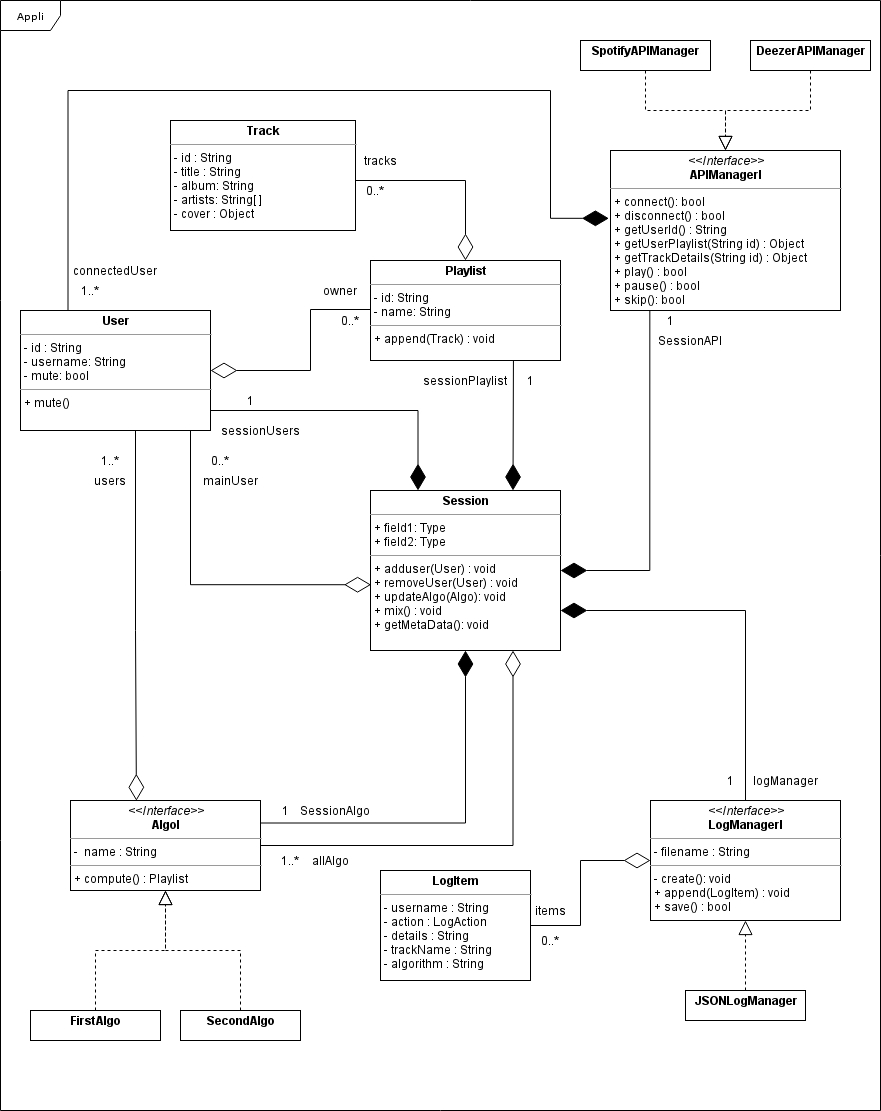
\includegraphics[width=\linewidth]{ressources/diagramme_classes.png}
			\caption{Diagramme de classes de l'application}
		\end{figure}
		\newpage
		\subsubsection{Architecture de l'application}\label{archi_log}
		\begin{figure}[h!]
			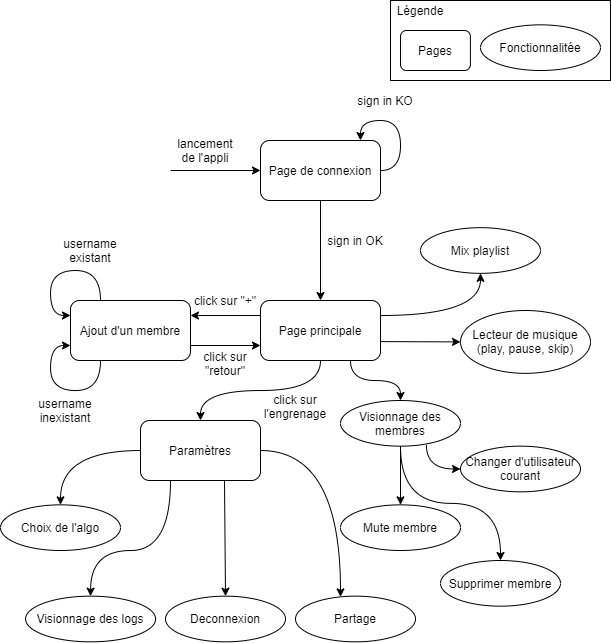
\includegraphics[width=\linewidth]{ressources/Architecture_Log.png}
			\caption{Architecture de l'application}
		\end{figure}
	
	    \newpage
		\subsubsection{Interface utilisateur}\label{interface_utilisateur}
		\begin{figure}[hb!]
			\centering
			\subfloat[Page de connexion]{{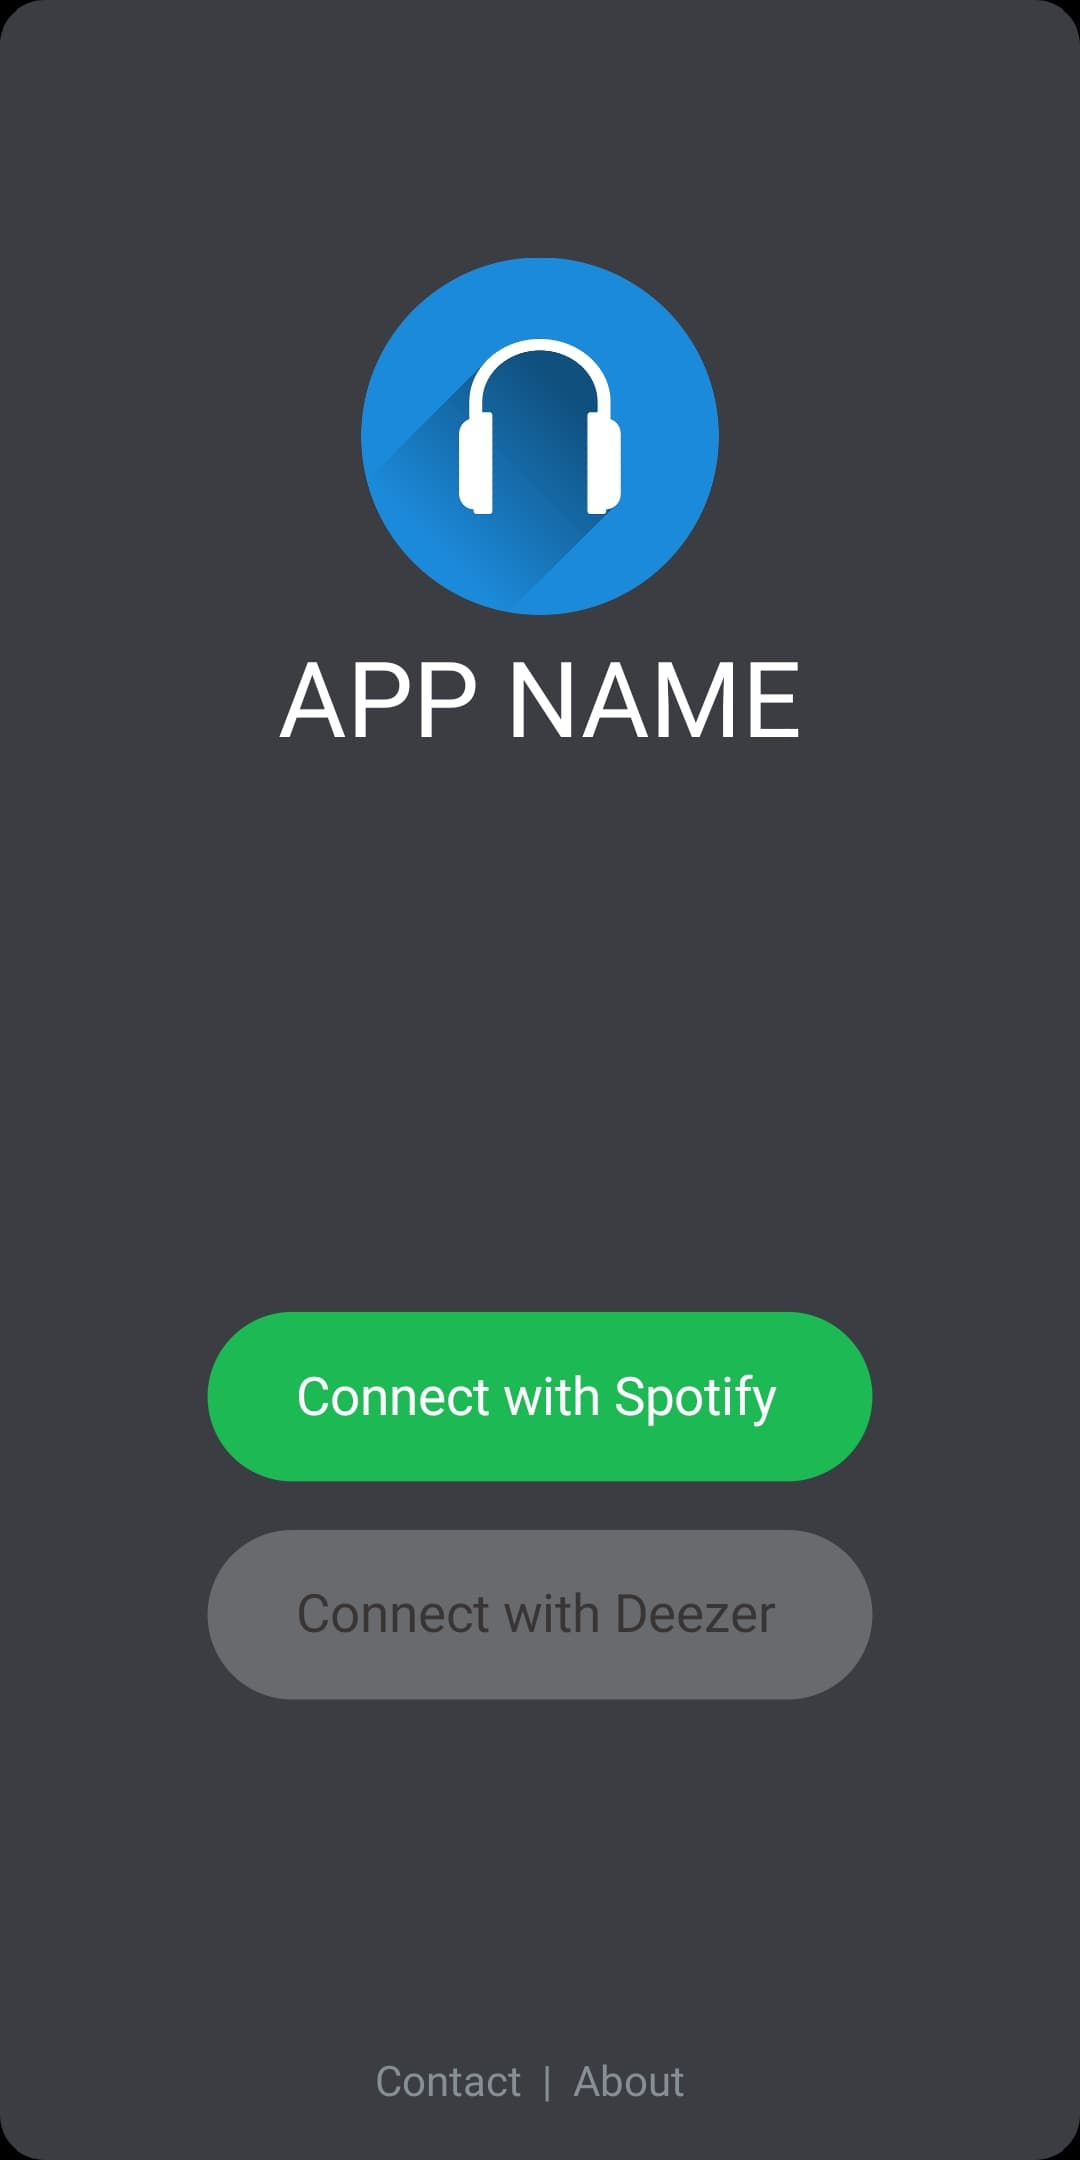
\includegraphics[width=4cm]{ressources/connection_page.jpg} }}\label{test}
			\subfloat[Page principale]{{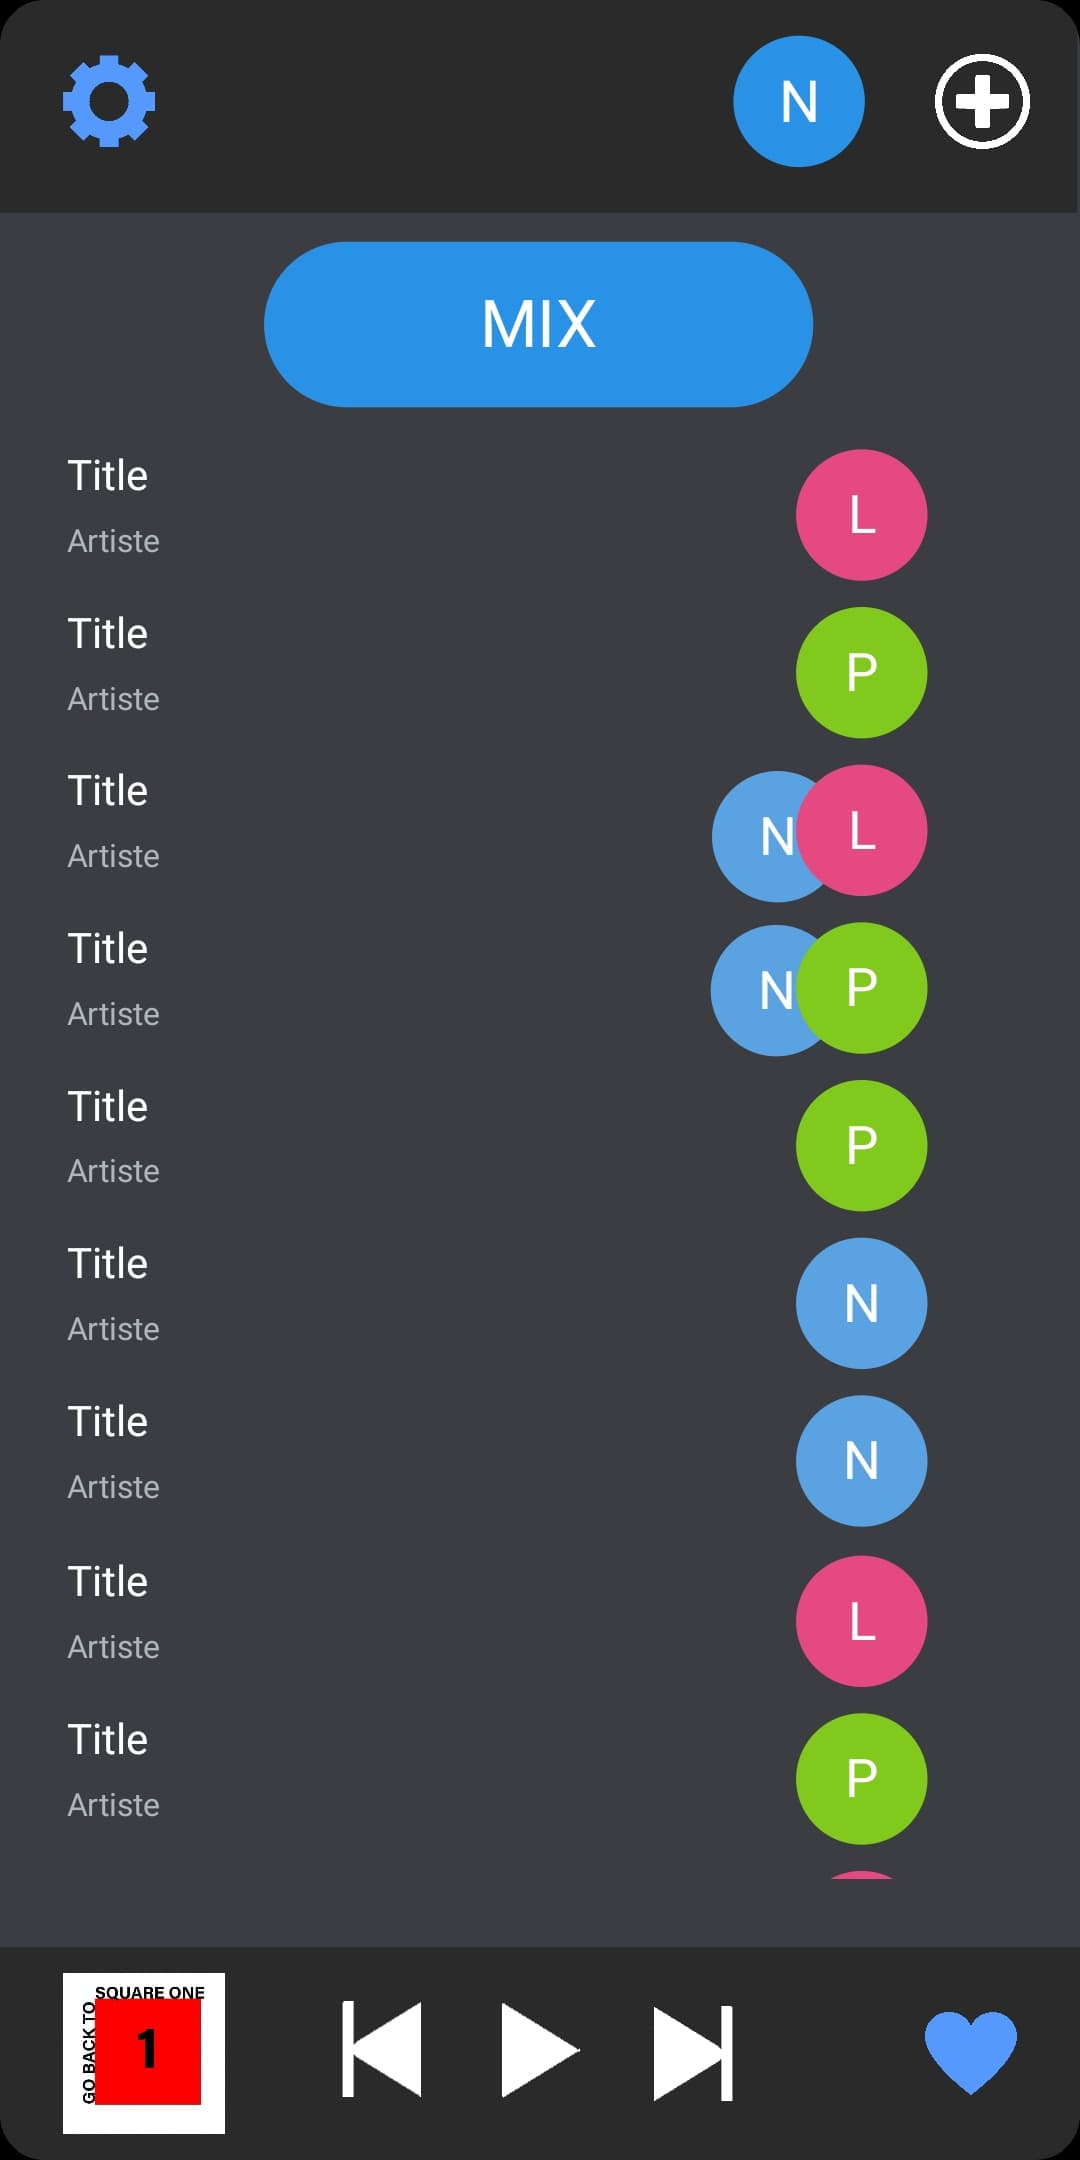
\includegraphics[width=4cm]{ressources/home_page.jpg} }}
			\qquad
			\subfloat[Page de gestion des utilisateurs]{{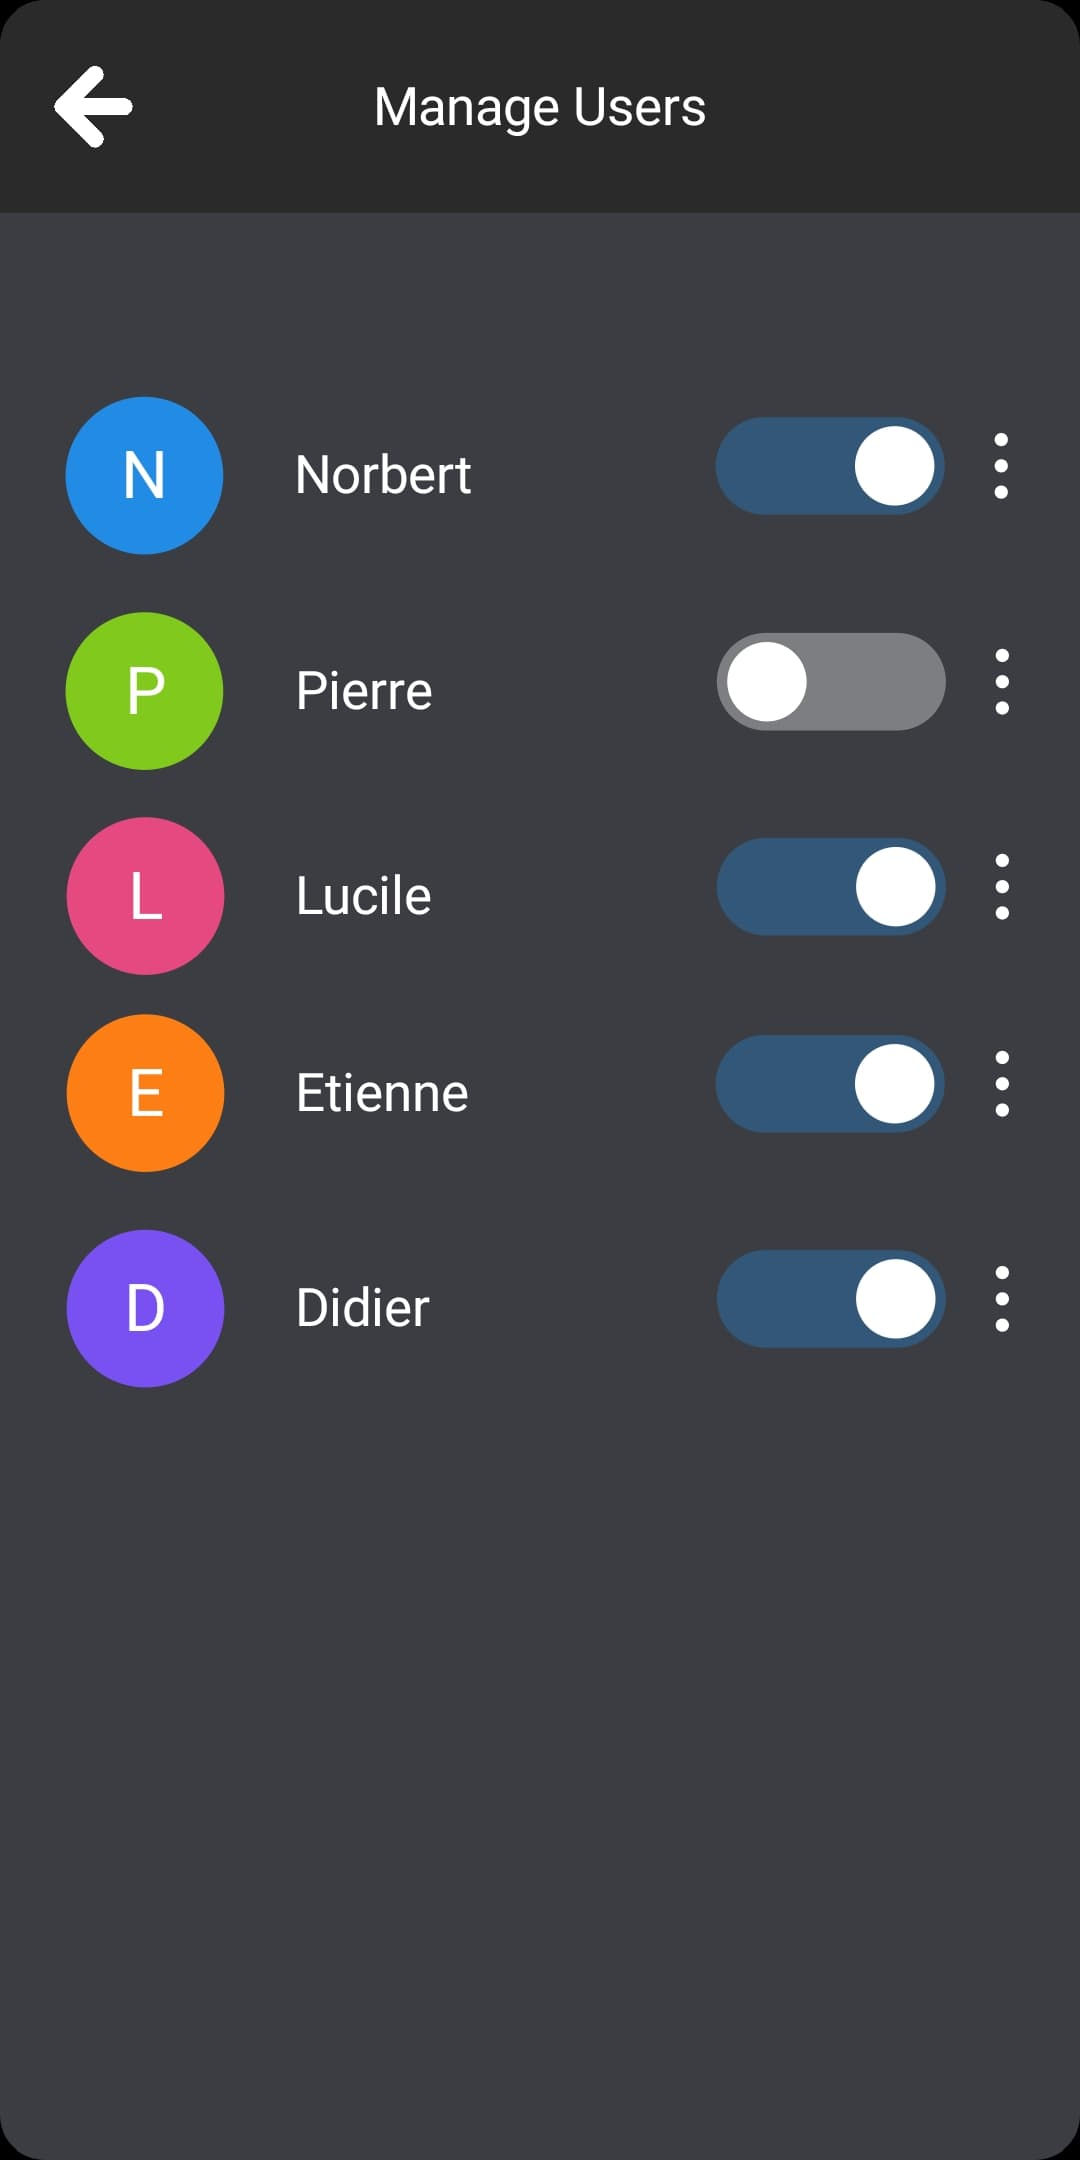
\includegraphics[width=4cm]{ressources/manage_user.jpg} }}
			\caption{Prototypes d'interface utilisateur}
			\label{fig:gui}
		\end{figure}
		\newpage
		\section{Gestion de Projet}
		\subsection{Décomposition des tâches}
		\paragraph{}
		Des besoins exprimés en \ref{besoins}. découlent des tâches que nous avons classées en fonction de leur nature : partie client (Front) et partie serveur (Back). Nous les avons aussi rangées par ordre de priorité de façon à simplifier l'écriture du diagramme de Gantt (cf. \ref{gantt})
								
		\subsubsection{Développement Front}
		\begin{enumerate}
			\item[]
			      \begin{description}
			      	\item[Essentiel :]
			      \end{description}
			\item Création de l'application\label{creation_item}
			\item Page principale générale\label{general_front_item}
			\item Page de connexion de l'utilisateur principal\label{connexion_front_item}
			\item Page principale : player\label{player_front_item}
			\item Page principale : playlist\label{playlist_front_item}
			\item Pop up d'ajout d'utilisateur secondaire\label{ajout_utilisateur_front_item}
			\item Page paramètres\label{parametres_front_item}
			\item Pop up d'accord de condition d'utilisation\label{conditions_front_item}
			\item[]
			      \begin{description}
			      	\item[Optionnel :]
			      \end{description}
			\item Pop up de suppression / mute d'utilisateur\label{utilisateur_gestion_front_item}
			\item Pop up de gestion avancée du player\label{player_sup_front_item}
		\end{enumerate}
		\subsubsection{Développement Back}
		\begin{enumerate}[resume]
			\item[]
			      \begin{description}
			      	\item[Essentiel :]
			      \end{description}
			\item Connexion/Authentification à l'API\label{connexion_item}
			\item Création de l'architecture objet\label{arch_item}
			\item Requêtes des playlists personnelles auprès de l'API\label{playlist_requete_item}
			\item Gestion de playlist\label{playlist_gestion_item}
			\item Gestion des algorithmes avec implémentation d'un algorithme naïf\label{algo_gestion_item}
			\item Gestion du player\label{player_gestion_item}
			\item Implémentation d'un premier algorithme\label{premier_algo_item}
			\item Récupérer les meta-données\label{data_item}
			\item Gestion des logs\label{log_gestion_item}
			\item Rédaction des conditions d'utilisation\label{condition_util_item}
			      			      			                  
			      \begin{description}
			      	\item[Conditionnel :]
			      \end{description}            
			\item Gestion de l'appli en background\label{background_item}
			\item Implémentation d'un second algorithme\label{second_algo_item}
			\item Gestion de l'utilisateur courant, avec identification des logs\label{utilisateur_courant_log_item}
			\item Gestion des requêtes en asynchrone\label{requete_async_item}
			\item Gestion de la déconnexion\label{deconnexion_item}
			\item Requêtes supplémentaires (likes, artistes préférés, ...)\label{requete_sup_item}
			\item Gestion de l'export des logs\label{export_log_item}
			      			      			                  
			      \begin{description}
			      	\item[Optionnel :]
			      \end{description}                 
			\item Gestion des utilisateurs (suppression, mute)\label{gestion_utilisateur_item}
			\item Gestion de l'export de playlist (vers Spotify)\label{export_playlist_item}
			\item Ajout des fonctionnalitéS supplémentaires du player (Se déplacer dans une musique)\label{player_gestion_sup_item}
			\item Adaptation à Deezer :\label{deezer_item}
			      \begin{itemize}
			      	\item Connexion/Authentification à l'API
			      	\item Requêtes des playlists utilisateures auprès de l'API
			      	\item Adaptation de playlist
			      	\item Gestion du player
			      	\item Récupérer les meta-datas
			      	\item Gestion des requêtes en asynchrone
			      	\item Gestion de la déconnexion
			      	\item Requêtes supplémentaires (likes, artistes préférés, ...)
			      	\item Gestion de l'export de playlist (vers Deezer)
			      \end{itemize}
		\end{enumerate}
		\subsection{Gantt} \label{gantt}
		\begin{center}
		\begin{tabular}{|*{3}{c|}|*{7}{c|}}
			\hline
			\diagbox[height=2\line]{Tâche}{Semaine} & 6 & 7 & 8 & 9 & 10 & 11 & 12 & 13 & 14    \\
			\hline
			\ref{creation_item}                      & P &   &   &   &    &    &    &    &       \\
			\hline
			\ref{general_front_item}                 &   &   & P &   &    &    &    &    &       \\
			\hline
			\ref{connexion_front_item}               &   &   & L &   &    &    &    &    &       \\
			\hline
			\ref{player_front_item}                  &   &   & J &   &    &    &    &    &       \\
			\hline
			\ref{playlist_front_item}                &   &   & E & E &    &    &    &    &       \\
			\hline
			\ref{ajout_utilisateur_front_item}       &   &   &   & P &    &    &    &    &       \\
			\hline
			\ref{parametres_front_item}              &   &   &   & J &    &    &    &    &       \\
			\hline
			\ref{conditions_front_item}              &   &   &   &   & E  &    &    &    &       \\
			\hline
			\ref{utilisateur_gestion_front_item}     &   &   &   &   &    &    & L  & L  &       \\     
			\hline
			\ref{player_sup_front_item}              &   &   &   &   &    &    &    & P  & P     \\           
			\hline
			\ref{connexion_item}                     & E & E &   &   &    &    &    &    &       \\
			\hline 
			\ref{arch_item}                          & L &   &   &   &    &    &    &    &       \\
			\hline
			\ref{playlist_requete_item}              & J &   &   &   &    &    &    &    &       \\
			\hline
			\ref{playlist_gestion_item}              &   &   & N &   &    &    &    &    &       \\
			\hline
			\ref{algo_gestion_item}                  &   & L &   &   &    &    &    &    &       \\
			\hline
			\ref{player_gestion_item}                &   & J &   &   &    &    &    &    &       \\
			\hline
			\ref{premier_algo_item}                  & N & N &   &   &    &    &    &    &       \\
			\hline
			\ref{data_item}                          &   & P &   &   &    &    &    &    &       \\
			\hline
			\ref{log_gestion_item}                   &   &   &   & L & L  &    &    &    &       \\
			\hline
			\ref{condition_util_item}                &   &   &   & N &    &    &    &    &       \\
			\hline
			\ref{background_item}                    &   &   &   &   & P  & P  &    &    &       \\
			\hline
			\ref{second_algo_item}                   &   &   &   &   & N  & N  &    &    &       \\
			\hline
			\ref{utilisateur_courant_log_item}       &   &   &   &   & J  &    &    &    &       \\
			\hline
			\ref{requete_async_item}                 &   &   &   &   &    & L  &    &    &       \\
			\hline
			\ref{deconnexion_item}                   &   &   &   &   &    & E  &    &    &       \\
			\hline
			\ref{requete_sup_item}                   &   &   &   &   &    & J  & J  & J  &       \\
			\hline
			\ref{export_log_item}                    &   &   &   &   &    &    & P  &    &       \\
			\hline
			\ref{gestion_utilisateur_item}           &   &   &   &   &    &    & N  &    &       \\       
			\hline
			\ref{export_playlist_item}               &   &   &   &   &    &    &    & N  & N     \\ 
			\hline
			\ref{player_gestion_sup_item}            &   &   &   &   &    &    & E  & E  &       \\         
			\hline
			\ref{deezer_item}                        &   &   &   &   &    &    &    &    & E,J,L \\   
			\hline
									
		\end{tabular}
		\end{center}
		\textbf{Remarque} : Les lettres dans les cases correspondent aux initiales des membres du projet. La double barre représente la première release.
						
		\section{Annexes}
				        
		\subsection{Annexe 1 : WebPlaybackState Object }
		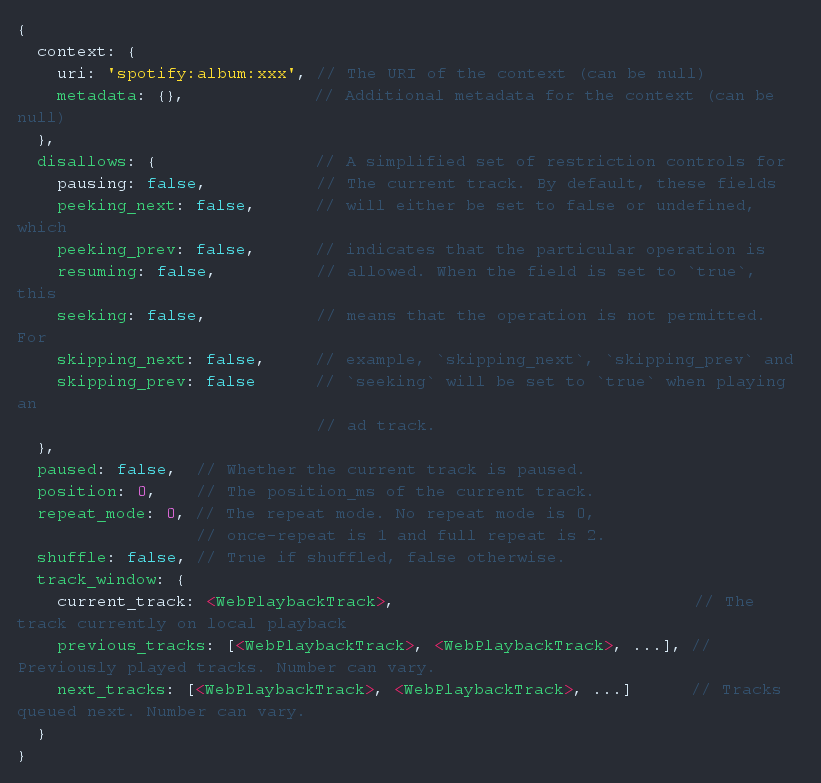
\includegraphics[width=\linewidth]{ressources/WebPlaybackState_Object.png}	\label{WebPlaybackState_Object}%
		\newpage
						
		\section{Bibliographie}
		\bibliography{references}
						
								
\end{document}